\pdfoutput=1
% \documentclass[a4paper,12pt,titlepage, twoside]{article}
\documentclass[a4paper,12pt,titlepage]{article}
\usepackage[english]{babel}
\usepackage[utf8]{inputenc}
\usepackage{amssymb,amsmath}
\usepackage{algorithm,algpseudocode}
\usepackage[title,titletoc]{appendix}
\usepackage{graphicx}
\usepackage{caption}
\usepackage{subcaption}
\numberwithin{figure}{section}
\usepackage{caption}


\begin{document}


% todo: compute Inception accuracy

\section{Introduction}
Estimated 80\% of the human data is in form of images or videos. ***citace*** There is a lot of useful information hidden, but it is still very complicated to gain it. Most of the information is still labeled manually by people, who make mistakes and are expensive. There is an incredible need for automated video processing in many branches of the industry. Being able to accurately detect and track vehicles can provide valuable data about transportation to governments. Reidentification and tracking objects over multiple cameras in real time can help reinforcement agencies to effectively fight crime. 

\subsection{Problem statement}
This thesis has been implemented for the company Good Vision s.r.o to be used in many South American cities for local reinforcement agencies. The cameras will be mounted directly to street lamps and will provide surveillance data to the police. The cameras have 360 degrees view thanks to their very short focal distances. 

If there was a crime committed and the person is driving away in a vehicle, an police officer marks the car and a set of algorithms introduced in this thesis will track the location of the vehicle in the city.

\subsection{Overview of methodology}

The whole thesis has been divided to subproblems and solved more or less separately. The model of the camera, it's parameters and transformations to the real world coordinates were be found as described int the section \ref{sec:lens}. The possibility of distributed computing directly in the cameras have been explored as described int the section \ref{sec:classical}. That included fast non deep learning set of algorithms for detection \cite{piccardi2004background}, tracking \cite{optical-flow} and classification \cite{haar} running on CPU. This approach could not be used directly because of some problems mentioned in the section. However, it was used for semi-supervised dataset generation. The approach for frame decomposition into multiple non distorted images have been explored in section \ref{sec:decomposition}, but for computational reasons not used in the final product. 

An annotation tool has been used as described in the section \ref{sec:ssd-dataset} for creating training and validation dataset. SSD\cite{liu2016ssd} neural network architecture has been used for object detection. This network has been extended for an additional input of temporal difference to better recognize moving objects and has been trained on NVIDIA GeForce GTX 1080.

Google Facenet \cite{facenet}, which was trained on a custom dataset from section \ref{sec:classical} has been used as a metrics of similarity between detections in section \ref{sec:facenet}. An overall model 


\subsection{Contribution}

***probrat osobne s vedoucim ***

The author of this thesis implemented several modules for this project.

\begin{itemize}
\item The calibration of the camera and estimation of the vehicle position.

\item Detector and tracker of vehicles using classical methods

\item Semi-supervised data generator

\item Improving, extending and training deep learning detector and connecting it with a provided tracker.

\item Training a neural network for vehicle similarity

\item Testing and comparing results.


\end{itemize}

implementing of classical model detections.
using the facenet model for similarities.
Improving the ssd model.

\section{Related work}

The computer vision field has made an incredible leap forward in last couple of years. Thanks to the increasing computational capabilities of computers and recent advancements in deep learning, we are able to do tasks, that we could not imagine. Image classification, location and detection are tasks, that have gone through an incredible evolution in the last 5 years. The face recognition, autonomous driving, surveillance and many more fields have been the driving force for computer vision. The tracking of objects over multiple cameras is valuable in retail, traffic monitoring and surveillance.

\subsection{Classification}

Image classification is a task, where given an image, one class has to be assigned from previously known set of classes. This is a hard task because of the variance in lightning, pose, rotation, scale, as well as intra class variation.  

Accuracy is usually measured as the proportion of correctly classified images in the test set. Two metrics are used. In top 1 accuracy only one prediction is made. In top 5 accuracy, 5 predictions are made and an image is considered to be correctly classified, if the correct class is among them.

To properly train, evaluate and compare models, several datasets, such as Mnist \cite{lecun-mnisthandwrittendigit-2010}, ImageNet \cite{deng2009imagenet}, or PASCAL VOC \cite{Everingham10} have been created.

Before the invention of convolutional neural networks, other classifiers were used. Classifiers in general can be divided into parametric and non parametric methods. The non-parametric ones require no training phase and the decision is based directly on the data. Most common method is the Nearest Neighbor approach \cite{boiman2008defense, zhang2006svm}. The parametric methods on the other hand require a training phase to find the parameters of the model, which can be in form of decision tree \cite{bosch2007image}, adaboost \cite{opelt2004weak}, or the most common Support vector machine (SVM).

The classification pipeline of SVM is such that a set of features is extracted and an Support Vector Machine (SVM) is applied. These features can have many different forms and can also be combined. A histogram\cite{chapelle1999support}, Bag of features \cite{lazebnik2006beyond, nowak2006sampling}, SIFT features \cite{yang2009linear, bicego2006use} or Haar features \cite{munder2006experimental} can be used.

Convolutional neural networks (CNNs) are the state of the art in image classification. They have been introduced in 1990's\cite{lecun1989backpropagation}, but only recently 

In 2012 AlexNet \cite{krizhevsky2012imagenet} won the ImageNet Large Scale Visual Recognition Challenge (ILSVRC) with the top-5 error being just a 15.4\%. This was a huge success compared to the second best with 26.2\% top-5 error rate and is considered to be the beginning of deep learning in computer vision. 

The paper ZFNet \cite{zeiler2014visualizing} in 2103 introduced some inside to how CNNs work by introducing De Deconvolutional Network could show various feature activations. It also outperformed the AlexNet on ImageNet by the top-5 error rate being 14.8\% and winning the ILSVRC 2013.

GoogLeNet/Inception won the ILSVRC 2014 with the incredible top-5 error rate of 6.67\%. the architecture was based on LeNet \cite{lecun1998gradient}, but introduced an inception module. this module eliminates all full-connected layers, greatly reducing the number of parameters.

The second best network in ILSVRC 2014 was the VGG Net \cite{simonyan2014very}. The depth of the network has been increased, but the number of parameters kept low thanks to very small 3x3 filters. The architecture is simpler than the Inception and it is widely used in transfered learning and as a detection backbones.

The Microsoft's ResNet\cite{he2016deep} introduced a 152 layers deep architecture. they are able to train the network thanks to the introduction of the residual connections. Part of the information passes through the layers unchanged. This helps to solve the vanishing gradient problem. With the top-5 error rate 3.57\% They surpassed the human accuracy winning the ILSVRC 2015.

The ResNet idea has been further developed. Wide ResNet\cite{zagoruyko2016wide} reduced the number of layers while widened the network. ResNeXt \cite{xie2017aggregated} is furthermore highly modularized and introducing new dimension called cardinality, which is more effective, than simply increasing the number of layers or their width. 

DenseNet \cite{huang2017densely} connects each layer to every other layers in front of it. This furthermore helps with the vanishing gradient problem and reducing the number of parameters. It outperforms ResNet while requiring less memory and computation.

The task of image classification is considered to be solved, but more research is being done. These image classification networks can be used as a backbone for other tasks, such as image detection, localization or segmentation.

\subsection{Detection}
\subsubsection{Vehicle detection}
There are many ways to detect vehicles, not just with cameras. One can detect changes in magnetic fields \cite{daubaras2012vehicle, caruso1999vehicle} or a laser scanner \cite{gate2009fast}.

Cameras are the most common sensor, but they can be also combined with a laser scanner \cite{wender20083d, premebida2007lidar} or a sonar \cite{kim2005front, wang2003online}. Sometimes a stereo vision \cite{bertozzi2000stereo, toulminet2006vehicle} can be used to gain a better model of the environment.

Lot of research has been done for detection of vehicles and people thanks to the recent advancements in autonomous driving. Many datasets have been created \cite{apollo-scape, madhavan2017bdd, RobotCarDatasetIJRR, ncarlevaris-2015a} for detecting vehicles, pedestrians and other objects from the vehicle's point of view. There is even a research for detecting vehicles by their shadow \cite{tzomakas1998vehicle}. The state of the art in vehicle detection using cameras is detecting each image independently using techniques described in the next section.


\subsubsection{Object detection}

In computer vision, the object detection is a specified task. The goal is to draw a bounding box around each object and assign it one class selected from a previously known set of classes. The accuracy is measured in mean Average Precision described in the section \ref{sec:mAP}. 

Before the rapid using of neural networks, various methods have been used for object detection. Haar features were used for detecting faces \cite{haar, lienhart2002extended, viola2004robust} and vehicles \cite{sun2002real}. For general object detection, the background subtraction \cite{piccardi2004background, horprasert1999statistical} or optical flow \cite{naoya1990optical, quenot1992orthogonal, chen2011tracking} described in the sections \ref{sec:bgs} and \ref{sec:optical-flow}. SIFT \cite{lowe2004distinctive} HOG \cite{girshick2014rich, wang2009hog, zhu2006fast, felzenszwalb2010object, dalal2005histograms} are also being used.

The big advancements came with the introduction of region proposal networks \cite{girshick2016region}. The R-CNN \cite{DBLP:journals/corr/GirshickDDM13} were the first to introduce this concept. R-CNN consists of two neural networks, one to propose the regions of interests and the second one to classify them. Their performance was mAP of 53.3\% on PASCAL VOC 2012 dataset. This was a huge success compared to the mAP of 43.3 \%\cite{carreira2012cpmc} the year before. However, R-CNN were very slow (47 seconds on GPU with the VGG16 \cite{simonyan2014very} network), thus were far from realtime video analysis. It requires a full AlexNet forward pass for each of the around 2000 proposals.

Improved and faster version Fast R-CNN \cite{girshick2015fast} achieved 68.4\% on PASCAL VOC 2012 with the VGG16 network while significantly increasing speed over 200 times compared to R-CNN. This was due to sharing computations over proposals and using a single network for the feature extractor, classifier and the regressor in one network. However, the selective search for the region proposals was found to be the bottleneck for the detection process.

The Faster R-CNN focused on exactly that. The feature extractor was also used for the region proposal network making the region proposal almost cost free. They also increased the learning speed, because only one CNN needed to be trained. Faster R-CNN with VGG-16 achieved 75.9\% mAP on PASCAL VOC 2012 dataset with just 7 fps on GPU. This is much closer to processing a realtime video.

The YOLO\cite{redmon2016you} performs 45 fps, mAP 63.4 on VOC 2007. It splits the image in a grid and predicts only two bounding boxes and class probabilities for a grid. However it struggles with detecting more small objects close to each other and would not be a good detector for vehicles from street camera. However,here have been some improvements to this network \cite{redmon2017yolo9000, redmon2018yolov3}.

Region convolutional neural networks, which create proposals and then classify them, are still too slow. The Single shot multibox detector (SSD) \cite{liu2016ssd} based on \cite{erhan2014scalable} leaves out the region proposals with the fixed number of regions. It was introduced in November 2016 and had an incredible 74.3\% mAP at 59 fps on VOC 2007. This network has been chosen for object detection in this thesis and will be described more in the section \ref{sec:ssd}. 

\begin{table}
\centering
\begin{tabular}{|l|c|c|c|c|c|}
  \hline
  &Faster R-CNN & Fast YOLO & YOLO & SSD300 & SSD512 \\
  \hline
  fps & 7 & 155 & 21 & 59 & 22\\
  \hline
  mAP & 73.2 & 52.7 & 66.4 & 74.3 & 76.8\\
  \hline
\end{tabular}
\caption{Results on PASCAL VOC2007 test.}
\end{table}

There has been lately many more architectures introduced, such as \cite{lin2017focal, li2017fssd, dai2016r} and many more are coming.


\subsection{Object tracking}

The previously described tasks process single images. Now the problem expands to a new discrete time dimension when processing video, but for now keeping just one video feed. The goal is to create a trajectory or a sequence of bounding boxes of an object. This task is difficult because of the illumination changes, partial and full object occlusions and the realtime processing requirements \cite{yilmaz2006object}. Almost all trackers assume, that the fps of the video is high enough, that the movements of the objects are smooth. 

The approach can be divided into a dense and a sparse method. 

The sparse method scans only pixels near by the tracked objects and tries to estimate their movement. This is especially good for tracking low number of objects. The object can be represented as a single point \cite{kale2015moving}, a bounding box \cite{comaniciu2003kernel, porikli2005multi, yilmaz2007object, elgammal2002background}, or a silhouette \cite{isard2001bramble}. Only the changes can be registered \cite{kale2015moving} or a robust reidentification \cite{veenman1998fast} can be used, which is more robust to occlusions. A statistical representation can be connected with a Kalman filter \cite{banerjee2008multi} or a particle filter \cite{zhong2012moving}. The movement is often estimated using sparse optical flow \cite{kale2015moving, mae1996object}. With the recent deep learning advancements, tasks as tracking are also being solved with deep neural networks \cite{bertinetto2016fully, held2016learning, gladh2016deep, gaidon2016virtual, lee2016globally}.

The dense methods for tracking receives a video and detections for each frame. This has the advantage, that the tracks can be created without explicitly manually selecting each object we want to track. However, these approaches are more computationally complex, since they require object detection. The try to connect the bounding boxes into a sequence of tracks. The main methods use Jaccard overlap \cite{tan2005introduction, benfold2011stable} and optical flow \cite{chen2011tracking}. This task can be complex because of the crossing tracks as well as false positive and false negative detections \cite{joshi2012survey, elgammal2002background}.












\subsection{Reidentification}
When an object leaves one camera and appears in another camera, the task is to recognize it. When positions and orientations of the cameras are not known, the location and speed of the detected objects can be used for obtaining the spatial relationships among the cameras \cite{makris2004bridging}. The key to reliable reidentification is to correctly model the relationships among the cameras, as well as to find a similarity metrics of the detected objects. When the cameras overlap, the key is to accurately estimate the position of the tracked object and match them \cite{khan2003consistent, krumm2000multi, zhao2005real}. The detected objects can look very differently on different scenes because of the different scaling, rotations and lighting conditions. The brightness transfer function can be estimated and compensated \cite{javed2005appearance, porikli2003inter}. 

When the camera's fields of view don't overlap, the task becomes much more challenging. The camera positions can be either known \cite{rahimi2004simultaneous} or unknown \cite{makris2004bridging}. For reidentification, mean a posteriori (MAP) is estimated, giving the probability of the detected object being the same \cite{javed2005appearance, huang1997object}. \cite{kettnaker1999bayesian} used a probabilistic Baesian model formulation with previously known transition functions. \cite{kang2003continuous} explored this system for controllable movable cameras. 




\section{Fish-eye camera model}
\label{sec:lens}

\begin{figure}[h]
\centering
\includegraphics[width=1\linewidth]{fig/stream1.png}
\caption{Frame of the provided video}
\label{fig:stream1}
\end{figure}

For correct estimation of the position of detected objects, it is crucial to find the relationships between the camera pixel position and the real world positions. 

The cameras have been provided by the Brazilian party and no technical parameters are available. The model of the camera and it's parameters must be found. A set of improvised requested calibration images have been provided.

\subsection{Scene localization}
\label{sec:scene_localization}
Before we find the model of the optics, we need to compensate for another hardware error of the camera. As can be seen in the image \ref{fig:stream1}, the scene is shifted to the left down. It is not even circle, but rather an ellipse. This is due to manufacturing uncertainty and this error is different on each camera. Since this project will be easily scalable, and it is not convenient to measure and set the parameters manually, an universal algorithm for detecting ellipse has been introduced.

The algorithm is based on optimization. It takes an image as an input and produces parameters of the ellipse. From observation, the ellipse can only be either the horizontal major axis or the vertical major axis ellipse. The equation \ref{eq:ellipse} of the ellipse is rather unusual, but it allows faster cost function evaluation.

\begin{equation}
\label{eq:ellipse}
\frac{(x-s_x)^2}{a} + \frac{(y-s_y)^2}{1} = r^2
\end{equation}

Now we need to find the parameters $s_x, s_y, a, r$.

The original image $I$ of the size $H, W$ and channels $I_1, I_2, I_3$ is transformed to a mask $M$ of the same size by thresholding the total sum of channels on 8 bit scale is grater or equal to 1. \cite{lukacs1997real}

\begin{equation*}
M_{x,y} = \begin{cases}
1 & if \quad \sum_{i=1}^{3} I_{i,x,y} \geq 1 \\
0 & otherwise
\end{cases}
\end{equation*}

The mask $M$ represents the scene by the pixels with the value 1 and the background by the pixels with the value 0. 

We create an additional mask $E(s_x, s_y, a, r)$ of the ellipse as 

\begin{equation*}
E_{x,y}(s_x, s_y, a, r) = \begin{cases}
1 & if \quad \frac{(x-s_x)^2}{a} + \frac{(y-s_y)^2}{1} \leq r^2 \\
0 & otherwise
\end{cases}
\end{equation*}

The cost function $C(M, E(s_x, s_y, a, r))$ penalizes the pixels that have been masked as the scene and lie outside the ellipse and the pixels, that have been masked as background and lie inside the ellipse.

\begin{equation}
C(M, s_x, s_y, a, r) = \sum_{x = 0}^{W-1} \sum_{y = 0}^{H-1} E_{x,y}(s_x, s_y, a, r) \cdot (1-M_{x,y}) + (1 - E_{x,y}(s_x, s_y, a, r)) \cdot M_{x,y}
\end{equation}

The algorithm could evaluate all combinations of parameters, but the number of searched parameters can be greatly reduced by searching in a coarse to to fine manner. 

In each step, a baseline is set and for each parameter a higher and a lower value by a constant is evaluated. The best value is selected and set as a new baseline for the next step and the constant is divided by two. The main idea is basically a binary search.


%
%\begin{verbatim}
%x, y, a, r := initialize_params()
%center_step, a_step, r_step := initialize_steps()
%
%while(not imporoving):
%    x_list := [x - center_step, x, x + center_step]
%    y_list := [y - center_step, y, y + center_step]
%    a_list := [a - a_step, a, a + a_step]
%    r_list := [r - r_step, r, r + r_step]
%    
%    x, y, a, r := select_best(x_list, y_list, a_list, r_list)
%    
%    center_step := center_step / 2
%    a_step := a_step / 2
%    r_step := r_step / 2
%    
%return x, y, a, r
%\end{verbatim}

The cost function evaluations can be run in parallel, which can speed up the process on multi-core CPU.

\subsection{Camera model}

To correctly localize object from the camera, we need to know the transformations between real world coordinates $x^w, y^w, z^w$ and the projection on the captured frame $x^f, y^f$. After applying the algorithm from \ref{sec:scene_localization}, we know, where in the frame the scene is projected. First, we will consider the circle model and at the end we will apply the transformation to ellipse. 

Computing in the cartesian coordinates is not very useful for optics. Instead, the world coordinates are chosen to be spherical and the frame coordinates are chosen to be polar. The world coordinates are in respect to the camera. 
The transformations between the world cartesian coordinates $x^w, y^w, x^w$ and the world spherical coordinates $r^w, \theta^w, \phi^w$ are as follows:

\begin{figure}[h]
\centering
\includegraphics[width=1\linewidth]{fig/sphere.png}
\caption{The spherical coordinates of the world}
\label{fig:sphere}
\end{figure}


\begin{equation*}
\begin{aligned}[c]
x^w &= r^w \cdot cos(\theta^w) \cdot sin(\varphi^w) \\
y^w &= r^w \cdot cos(\theta^w) \cdot cos(\varphi^w) \\
z^w &= r^w \cdot sin(\theta^w) \\
\end{aligned}
\qquad,\qquad
\begin{aligned}[c]
r^w &= \sqrt{(x^w)^2 + (y^w)^2 + (z^w)^2} \\
\theta^w &= arcsin\Big(\frac{z^w}{r^w}\Big) \\
\varphi^w &= arctan\Big(\frac{y^w}{x^w}\Big) \\
\end{aligned}
\end{equation*}



The detected scene circle has the radius of $R$ pixels and the center at pixels $s_x, s_y$. The transformations between cartesian frame coordinates $x^f, y^f$ and the polar frame coordinates $r^f, \theta^f$ are:

\begin{equation*}
\begin{aligned}[c]
x^f &= s_x + R \cdot r^f \cdot cos(\varphi^f) \\
y^f &= s_y + R \cdot r^f \cdot sin(\varphi^f) \\
\end{aligned}
\qquad,\qquad
\begin{aligned}[c]
r^f &= \sqrt{(x^f - s_x)^2 + (y^f - s_y)^2} \\
\varphi^f &= arctan\big{(}\frac{y^f - s_y}{x^f - s_x}\big{)}
\end{aligned}
\end{equation*}

Next, we need to find the transformations between the world spherical coordinates $r^w, \theta^w, \phi^w$ and the frame polar coordinates $r^f, \theta^f$, but there are some nice properties:

\begin{itemize}
\item The $\varphi$ are the same, i.e. $\varphi^w = \varphi^f$.
\item The transformations do not depend on $r^w$. The projection depends only on the direction, not on the distance from camera.
\end{itemize}

With this knowledge, we need only to find the transformation of $\theta^w$ and $r^f$. We need to find a function $f$, such as 
\begin{equation}
\begin{aligned}
\theta^w &= f(r^f) \\
r^f &= f^{-1}(\theta^w). \\
\end{aligned}
\end{equation}

There are many models for finding $f$. 

\begin{itemize}
\item The linear model: $f(r^f) = FOV \cdot r^f$
\item The tangent model: $f(r^f) = FOV \cdot \tan(r^f)$
\item The sinus model: $f(r^f) = FOV \cdot \sin(r^f)$
\end{itemize}

With each model, we need to find the one parameter $FOV$, which is the field of view of the camera.

There was no access to the cameras, so the standard calibration using mesh could not be used. Instead, a set of marks was provided as shown in the picture. These marks are exactly 2 meters apart and are enough to estimate the function $f(r^f)$.

\begin{figure}[h!]
\centering
\includegraphics[width=1\linewidth]{fig/calibration.png}
\caption{The provided calibration data}
\label{fig:calibration}
\end{figure}


\subsubsection{Linear model}

This is the simplest one. The real world angle is proportional to the distance from the center on the image. 

\begin{equation}
\theta^w = f(r^f) = FOV \cdot r^f
\end{equation}

Fitting of the model is shown in the fig.\ref{fig:linear_model}

\begin{figure}[h!]
\centering
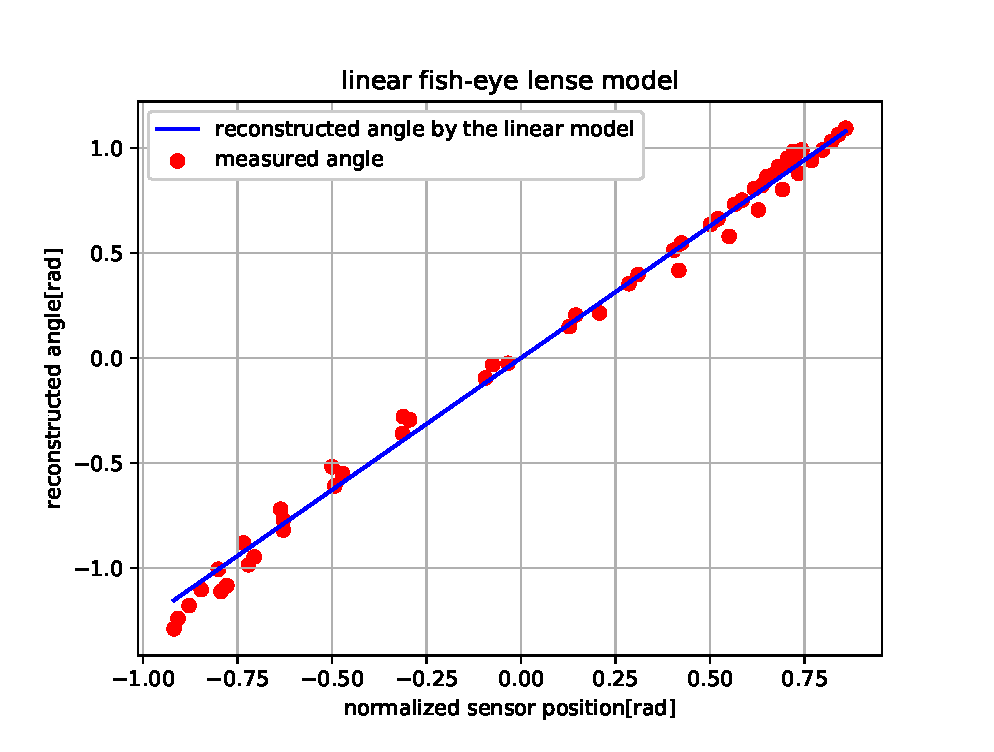
\includegraphics[width=1\linewidth]{fig/linear_model3.eps}
\caption{The linear model of the lens}
\label{fig:linear_model}
\end{figure}

The linear model somehow estimates the real one, but not that well.

\subsubsection{Tangent model}

This is a more complicated model, which is based on the pinhole camera model.

\begin{equation}
\theta^w = f(r^f) = \theta^w \cdot FOV,
\end{equation}

Fitting of the model is shown in the fig.\ref{fig:linear_model}

\begin{figure}[h!]
\centering
\includegraphics[width=1\linewidth]{fig/tan_model2.eps}
\caption{The linear model of the lens}
\label{fig:linear_model}
\end{figure}

This model represents the camera optics much better and was chosen to be the final one.

\subsection{The city coordinate system}

There is many ways how to represent real world for representing the car in the city. The most obvious one would be represent the position by longitude, latitude and elevation. This would be correct, but not very practical. Since the distances between same circles of latitude and longitude are different, this would need more complicated transformations and there is a simpler model. 

Since we care only about only one city, we will use a city cartesian coordinate system $(x^c, y^c)$. We can choose any position and rotation of the coordinate center. All we need to know is the relative translations and rotations of each camera $(\Delta x, \Delta y, \Delta\phi)$ to the city coordinate system. For simple transformations we will use homogeneous coordinates, which are in form of $(x, y, 1)^T$. 


A point from a camera coordinate system $(x^w, y^w)$ is transformed to the city coordinate system $(x^c, y^c)$ as
\[
  \begin{bmatrix}
    x^c \\
    y^c \\
    1
  \end{bmatrix}
   = 
  \begin{bmatrix}
    cos\Delta\phi & -sin\Delta\phi & \Delta x\\
    sin\Delta\phi & cos\Delta\phi & \Delta y\\
    0 & 0 & 1
  \end{bmatrix}   
  \cdot 
  \begin{bmatrix}
    x^w \\
    y^w \\
    1
  \end{bmatrix}
\]








\section{Detection and tracking on CPU}
\label{sec:classical}
The final system needs be easily scalable and a particular system architecture has been explored. If the detections and tracking were computed on-board of the cameras, that would help greatly. There would be much less communication needed. Instead of transferring whole video streams, only some meta-data would be sent. That would include: 

\begin{itemize}
\item Time stamps of a frames.
\item Locations of objects and their classes.
\item Some description vector of the detections.
\item Detections clustered to tracks.
\end{itemize}

This system could be greatly distributed sending packets of information among only the cameras that the information is relevant to.

However this has some downfalls, mainly in computational manner. Each camera would have to be equipped either with a capable computational unit. The detections, tracking and similarities would all have to be computed onboard. Since it is not possible to have a GPU in every lamp for many reasons, for example it is a very wet environment, usage of neural networks would not be possible. This section introduces non deep learning approach for detection, tracking and classification, that could run on CPU.



\subsection{Background subtraction detection}
\label{sec:bgs}

Probably the best classical detection methods from static videos, that can be computed in real time on limited hardware, are based on the background subtraction algorithm \cite{piccardi2004background}. The main idea is creating a model of the scene without the objects that we want to detect and then subtracting the current frame and by thresholding determine, where the vehicles are. This simple approach does not work very well and some improvements need to be made. 

For the background subtraction procedure, a model of the background has to be found. For our purposes we need to know, how the road looks like without any vehicles and people. This can't be done by simply waiting for such a case, because the traffic is usually quite high. Instead, we need to figure out the background from multiple frames. 

\cite{horprasert1999statistical, zivkovic2006efficient}

The algorithm has been implemented in opencv \cite{opencv}. The background is usually created by the mean over several images called running gaussian average \cite{wren1997pfinder}. The idea is to estimate a gaussian to each pixel independently. Each pixel is updated with each new frame as a weighted sum. The background looks like a photo with a long exposition and the lane. In places, where vehicles drive, are colored lines as shown in the figure \ref{fig:cut_mean}. When computed the difference from a video frame to such a background model, as shown in the figure \ref{fig:threshold_mean}, the places, where usually cars drive, can have high values. This can be bad for creating a mask by thresholding, because a higher thresholding constant has to be set.

\begin{figure}
    \begin{subfigure}[Sample1]{0.5\linewidth}
        \includegraphics[height=37mm]{fig/background_mean_crop.png}
        \caption{Mean model}
        \label{fig:cut_mean}
    \end{subfigure}
    \qquad
    \begin{subfigure}[Sample1]{0.5\linewidth}    
        \includegraphics[height=37mm]{fig/background_med_crop.png}  
        \caption{Median model}
        \label{fig:cut_med}  
    \end{subfigure} 
    \caption{Background model created by the mean and the median approach.}
\end{figure}

The background model changes with every new frame. In the first iteration, the background $B_0$ is just the first frame $F_0$. The background in next iteration is just the weighted sum of the  current frame and the background model in the previous iteration.

\begin{equation}
B_n = \alpha \cdot F_n + (1 - \alpha) \cdot B_{n-1}
\end{equation}

This algorithm is very fast and can be highly parallelized and computed on graphics cards. The picture having $N$  pixels, the complexity of this standard background subtraction algorithm is  $O(N)$.



\begin{figure}
    \begin{subfigure}[Sample1]{0.5\linewidth}
        \includegraphics[height=37mm]{fig/threshold_mean_crop.png}
        \caption{Mean}
        \label{fig:threshold_mean}
    \end{subfigure}
    \qquad
    \begin{subfigure}[Sample1]{0.5\linewidth}    
        \includegraphics[height=37mm]{fig/threshold_med_crop.png}
        \caption{Median}
        \label{fig:threshold_med}    
    \end{subfigure} 
    \caption{The difference between the frame and a background shown in a gray-scale.}
\end{figure}

An improved way of acquiring background model has been used, which greatly improves the quality of current background subtraction methods. A simple change of taking the median instead of the mean at each pixel position gives much better estimation of the background \cite{bgs-med1, bgs-med2}. The algorithm keeps a queue of $K$ images in a memory and with each incoming frame it puts it in the database and for each pixel it computes a median from the queue. This algorithm can be implemented with the complexity $O(N \cdot log(K))$, if we insert each pixel from an incoming frame to a sorted structure. In reality, for small $K$ this would slow the algorithm, because in opencv and numpy there is a great support for working with the whole images. This approach is simply compute the median over all the images from the queue. The complexity is $O(N \cdot K \cdot log(k)).$ The $K$ has been set to 35. The histogram of a particular pixel position over the queue is show in the figure \ref{fig:pixel_hist}.


This turns out to work much better, but still has it's limits. If the traffic is very high and vehicles occupy in average more than half of the ground, the background model will fail, but mean approach would fail as well. 

\begin{figure}[h]
\centering
\includegraphics[width=1\linewidth]{fig/pixel_hist.eps}
\caption{The histogram of a particular pixel over 100 images with computed medians}
\label{fig:pixel_hist}
\end{figure}

Some more complicated models based on unsupervised learning, such as clustering or taking the most frequent bin from histogram for each pixel position could be used, but they would be computationally too complex and would not be practical for realtime video.

The difference between background model and the current frame is very noisy and some filtration has to be made. Before subtraction, the background and the frame has been filtrated with a gaussian filter with the size 3x3 for smoothing. This compensates for the camera vibrations. Then smoothed again with the filter 11x11. This serves as an apriori probability. The idea is, that if there are big differences in the neighboring area, it is a higher probability of the pixel belonging to the car. This also helps to detect gray and black cars, which have similar color to the road. Another advantage is, that this greatly reduces noise and helps to detect vehicles as whole.

This differential image is thresholded and a mask is obtained as shown in the figure \ref{fig:mask_area}. Each blob is presented with a contour and they are thresholded once more by the area. The resulted blobs become detections and a bounding box is created.

\begin{figure}
    \begin{subfigure}[Sample1]{0.5\linewidth}
    	\includegraphics[height=85mm]{fig/frame_cropped.png} 
        \caption{A frame for detection}
        \label{fig:frame_for_detection}   
    \end{subfigure}
    \qquad
    \begin{subfigure}[Sample1]{0.5\linewidth} 
    	\includegraphics[height=85mm]{fig/mask_area.png}
        \caption{The detections and areas of contours.}   
        \label{fig:mask_area}
    \end{subfigure} 
    \caption{The background subtraction detection algorithm.}
\end{figure}

The background must be continuously adapting to the scene, but the rate of adapting is crucial. If the background is changing too slowly, it will not work very well with changes of lightning from coming clouds, etc. If the background adapts too fast, it will start to contain cars, that stop at the cross section and when the cars leave, this will become a new false detection. From experiments, there is no optimal adapting rate and it depends on the scene, weather and even then these problems will not completely disappear. One small advantage is filtering detections while adapting background.

Background subtraction is a very fast detection algorithm and when having perfect conditions, it is very accurate and The bounding boxes are more precise than most deep learning approaches.

Unfortunately it has many downsides. 

\begin{itemize}
\item Moving trees and their shadows create false positives.
\item Overlapping vehicles are detected as only one.
\item It works bad in high traffic, because it can't create a correct background model.
\item It is very sensitive to changes of lightning, such as moving clouds.
\item It is very sensitive to correct setting of hyper-parameters.
\end{itemize}

Most of these points relate to changing background. Especially if the scene is partially cloudy and the lightning changes a lot, the background model needs to adapt quickly. On the other hand, if in the scene is a traffic light, cars spend a lot of time on one spot and could be incorporated to the background model. Not only the car will not be detected, but a false positive will be detected when the car leaves.

For these problems, background subtraction alone can't be used as a good detector, but on perfect scenes  it can be very useful for collecting high quality training data for neural networks detectors, as described in the section \ref{...}.

\subsection{Optical Flow tracking}
\label{sec:optical-flow}
The detections have been described in section \ref{sec:bgs}. Having only the detections for each frame does not give us that much information. We need to connect these detections to a track.

A custom set of algorithms has been implemented in opencv\cite{opencv} for extending the background subtraction algorithm to tracking. Optical flow \cite{optical-flow} is used for a motion estimation in a video. It pairs pixels in two subsequent frames. In other words, it is a discrete 2D vector field, where each vector is a displacement vector showing the movement of points from first frame to second.

The computation of optical flow over the whole image is usually a very expensive procedure. The method used is Lucas-Kanede method \cite{lucas-kanede}. 

***desctiption, equations, dense/sparse? ***


This algorithm is not used on whole image. That would be computationally too expensive and would not be feasible for limited computational resources and realtime system. Instead, each detection is extended for a one optical flow point. In the next frame, this point will move with the object. Each detection is characterized through this point. 

This extends the detector for object tracking and partially solves the problem of two overlapping vehicles. If two vehicles drive close to each other, background subtraction would start to treat them as one object. This improved model will detect this situation and try to keep the bounding boxes on the different vehicles. 

In first experiments, when a new detection appeared, the position of the optical flow point was selected with the Shi-Tomasi \cite{shi-tomasi} algorithm, which is an improved version of the Harris corner and edge detector \cite{harris}. It tries to find some features, that have high gradient and will be easier to track, rather than selecting just the muddle of the bounding box.



In a perfect scenario the algorithm could be used without further improvements. However in real world scenario, false positives, as well as false negatives detections must be dealt with. Furthermore trees and lamps also complicate the situation greatly. When a vehicle drives behind some sort of a pillar, the optical flow point can not be matched with a next frame and stays on the same place in the frame. When the vehicle completely passes, the tracking is lost. A feature had to be added, which is an additional centering of the optical flow point to the middle of the bounding box. with each new frame, the optical flow point moves with the vehicle, but is also moved towards the middle of the bounding box. This solves the issues of the pillar obstacles, but excludes using the Shi-Tomasi and Harris features. 


The tracking algorithm has been described by a set of rules. The main ones are:
\begin{itemize}
	\item If an optical flow point is outside the background subtraction mask, it becomes a 'zombie'.
	\item If a background subtraction detection is without an optical flow point and there is no 'zombie' in the detection, optical flow point is created in the middle of the bounding box. 
	\item If a zombie is not recovered in 10 frames, it disappears. 
	\item If there are more optical flow points in one background subtraction detection, the bounding boxes continue movement with a low pass filter.
	\item The optical flow points are forced to the middle of the bounding box. This solves the problem of the detection being put on the front of the car while coming and due to noise later being outside the bounding box, when the vehicle is viewed from a side. 
\end{itemize}

These improvements work surprisingly well and solve the tracking problem to some extent. If vehicles overlap completely, this approach will fail, but so will most of the other ones. 

\subsection{classification}

In the frames, there are many objects detected and need to be classified. The most important distinction is between a person and a vehicle. 

A simple classifier has been introduced using 87 distinct Haar features.  Each Haar feature is a difference of average brightness level in two different rectangles in the image. The SVM classifier has been trained on 8144 images of cars and 10567 images of people. The test set split ratio was 0.2 reaching the accuracy 0.842. That is quite a good score without using neural networks, but not good enough for the final project.

The training and testing data have been acquired by developed semi-supervised data annotator based on the detector and tracker introduced in the section \ref{sec:data-generation}.

\subsection{Semi-supervised data generation} 
\label{sec:data-generation}

Standard annotation approaches for image detection training need the annotator to draw a rectangle and assign it a class for every detection. This is very time consuming and therefore costly. Video is usually around 25 frames per second, so to annotate a minute of video means annotate a 1500 images. This process can be made easier by skipping some frames and moving the bounding boxes around. For the skipped frames linearly approximate the movement of the objects. This can speed up the process, but it still takes a very long time. 


The algorithms introduced in this section can not be used for the final product, mainly because of the problems described in the section \ref{sec:bgs}. However that does not mean, that this can not be used for other purposes. As mentioned before, it works very well on easy scenes. The bounding boxes are precise and this can help the annotator to annotate scenes faster and more precisely, than standard approaches. the annotator is presented a dialog as shown in the figure \ref{fig:labeling}. That includes the whole track, which is annotated through one click. 


\begin{figure}[h!]
\centering
\includegraphics[width=0.5\linewidth]{fig/omni_labeling.png}
\caption{The dialog from the annotation tool.}
\label{fig:labeling}
\end{figure}


Because of the not perfect classifier, it is not used. Instead, the annotator selects the class or to throw the whole track away.


and can alswhich detections will be used


% corello

\section{Detection and reidentification}
tried inception rcnn, but not working directly.

***A processing of a single frame needs to be perfected. That includes detection and classification. Detection is in form of a bounding box. Each detection in a single frame needs to be classified into several classes. When we have a detections and classifications over a sequence of frames, a tracking needs to be implemented. That means connecting the bounding boxes into sequences, where each sequence of bounding boxes represents a trajectory of a vehicle. ***


\subsection{Neural networks for classification}
\label{sec:neural_networks_classification}
The Neural networks have been the state of the art for the classification. Furthermore they are used as the backbone for detection networks.

\subsubsection{intuition}

\subsubsection{*** conv layers, ..., ?}
\subsubsection{VGG512}

\subsection{SSD network}
\label{sec:ssd}

The state of the art in detection is at the time the Single Shot MultiBox detector \cite{liu2016ssd}. This network provides accurate realtime object detections (74.3\% mAP at 59fps on VOC2007 on GPU). They achieve much faster speed, compared to previous Faster R-CNN (7 fps on GPU) thanks to eliminating the bounding box proposals. Since the SSD architecture is much simpler and compact, than R-CNN architectures, the training is performed end to end on a single model, instead of training multiple networks for region proposal, classification and bounding box regression.

\subsubsection{Architecture}

\begin{figure}[h!]
\centering
\includegraphics[width=1\linewidth]{fig/SSDvsYOLO.png}
\caption{Comparison of the SSD\cite{liu2016ssd}(300x300) and YOLO\cite{redmon2016you}(448x448) architectures.}
\label{fig:ssd_vs_yolo}
\end{figure}

The SSD network uses one feed forward flow to produce a fixed number of bounding boxes and their probability for each class. The early layers are sometimes called a base network or a backbone. They are a classical architecture for image classification. 

Some additional layers have been added on top of the base network show in fig. \ref{fig:ssd_vs_yolo}. Multi-scale feature maps for detection are convolutional layers that progressively decrease their size and allow cheap detections of multiple scales. Convolutional predictors for detection can from feature maps of size $m \times n$ with $p$ channels can predict scores for categories or the offsets for each $3 \times 3$ element  using small kernels of $3 \times 3 \times p$. With decreasing feature maps, the predictions relate to different object scales. The bounding boxes offsets are measured relative to the each feature map location. 

\subsubsection{Default boxes and aspect ratios}
Each feature map cell, from the feature maps at the end of the network, is associated with a set bounding boxes. They differ in shape and scale as shown in the figure \ref{fig:ssd8}. Since the feature maps are computed from convolutions and max pool layers, the bounding boxes regularly tile the input image as shown in the figure \ref{fig:ssd8} with fixed positions.

A prediction of a probability of each class and predicted offset of the the bounding box is computed. The offsets are given relative to the associated fixed position of the bounding box as shown in the figure \ref{fig:ssd4}. For predicting $k$ shapes and $c$ classes with 4 numbers representing the translations $\Delta(cx, cy, w, h)$, we need $k(c+4)$ filters for each feature map cell and for one $m \times n$ feature map layer we need $mnk(c+4)$ filters. The default boxes are similar to anchor boxes in Faster R-CNN with the difference, that SSD uses multiple feature maps for different object scales. 


\begin{figure}
    \begin{subfigure}[Sample1]{0.3\linewidth}
    	\includegraphics[height=35mm, width=35mm]{fig/ssd_dog_cat.png} 
        \caption{SSD prediction}
        \label{fig:ssd_detection}   
    \end{subfigure}
    \quad
    \begin{subfigure}[Sample1]{0.3\linewidth} 
    	\includegraphics[height=35mm, width=35mm]{fig/ssd_feature_map.png}
        \caption{8 $\times$ 8 feature map.}   
        \label{fig:ssd4}
    \end{subfigure} 
    \quad
    \begin{subfigure}[Sample1]{0.3\linewidth} 
    	\includegraphics[height=35mm, width=35mm]{fig/ssd_4_feature_map.png}
        \caption{The predicted offsets.}   
        \label{fig:ssd8}
    \end{subfigure} 
    \caption{The background subtraction detection algorithm.}
\end{figure}

\subsubsection{Training}
With each training image, the ground truth boxes need to be assigned to a default bounding box. The ground truth box is matched to all default boxes, which have the Jaccard overlap higher than 0.5. This is more robust, than picking only the one box with the highest overlap as in MultiBox \cite{erhan2014scalable}. After that, the training is performed end to end by a standard backpropagation. 

The training phase also includes a positive and a hard negative mining. Not all predicted boxes participate on training. Most of the predicted boxes are usually negatives. The backpropagation is on all the boxes matched with ground truth box as well as the negatives with lowest score for background. This is called hard negative mining and it speeds up the convergence. The negatives are picked with the ratio 3:1 to the positives.





\subsection{Facenet}
\label{sec:facenet}




\section{Implementation}

\subsection{Image decomposition}
\label{sec:decomposition}

\subsection{Dataset}
\label{sec:ssd-dataset}
standford \cite{standford} cars dataset




\section{Evaluation}



\subsubsection{Mean average precision.}
\label{sec:mAP}
Mean average precision (mAP) is the most used metrics for object detection problem. The advantage is, that it does not depend on the selected confidence threshold, but only on the IoU threshold. This metrics is not constrained only for object detection problems in vision, but can be used for all detection problems. 

The algorithm for computing mAP runs for all thresholds. Given an arbitrary threshold, the predicted bounding boxes are those, whose confidence exceeds it. If there is a high IoU of a ground truth box and some predicted bounding boxes having the same class, the predicted box with the highest confidence is matched and considered true positive($TP$) and no other box can be matched with the ground truth bounding box. If a predicted bounding box is not matched with any ground truth bounding boxes, it is considered false positive($FP$). If a ground truth bounding box is not matched with any predicted bounding box, it is considered a false negative($FN$).

Precision($P$) corresponds to what portion of ground truth boxes have been matched. With lowering the threshold, it can only increase, since more ground truth bounding boxes will be matched.
\begin{equation}
P = \frac{TP}{TP + FP}
\end{equation}

Recall($R$) corresponds to what portion of predicted bounding boxes have been matched. 
\begin{equation}
R = \frac{TP}{TP + FN}
\end{equation}

The precision-recall curve in the Fig.\ref{fig:precision-recall} shows the dependency of precision and recall. The higher the precision, the lower the recall. The area below the curve is called average precision($AP$) and the mean over all classes is called mean average precision($mAP$).

\begin{equation}
mAP = \frac{1}{|C|} \sum_{c \in C} AP_c
\end{equation}

where $C$ is the set of classes.

\begin{figure}[H]
\centering
\includegraphics[width=1\linewidth]{fig/precision-recall.png}
\caption{Example of precision-recall curve}
\label{fig:precision-recall}
\end{figure}







\bibliographystyle{plain}
\bibliography{ref}{}
\cleardoublepage
\clearpage

\end{document}